Der euklidische \index{Euklid} Algorithmus \index{Algorithmus} \footnote{ \url{ https://de.wikipedia.org/wiki/Euklidischer_Algorithmus}} ist ein Algorithmus aus dem mathematischen Teilgebiet der Zahlentheorie. Mit ihm lässt sich der grösste gemeinsame Teiler \index{Grösster gemeinsamer Teiler} zweier natürlicher Zahlen berechnen. 

\begin{wrapfigure}{r}{5cm}
  \vspace{-14pt}
  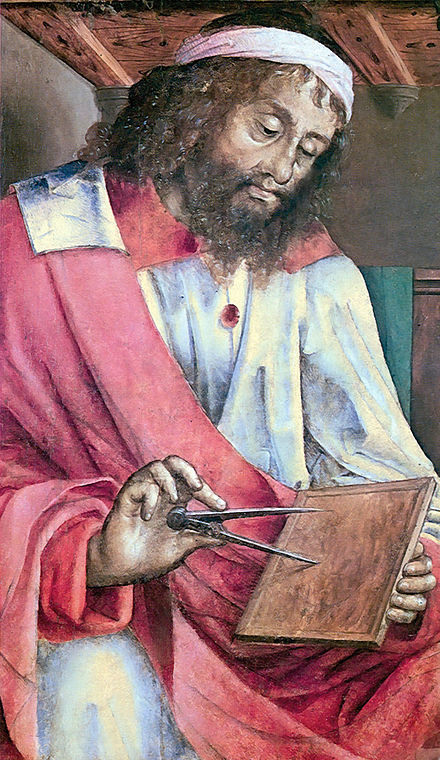
\includegraphics[width=5cm]{./screenshots/euklid.jpg}
  \vspace{-14pt}
  \caption{Euklid}
  \label{fig:euklid}
  \vspace{-30pt}
\end{wrapfigure}


Das Verfahren ist nach dem griechischen Mathematiker Euklid benannt, der es in seinem Werk „Die Elemente“ beschrieben hat.

\textbf{Klassischer euklidischer Algorithmus:}\index{Euklid!klassischer Algorithmus} Euklid berechnete den grössten gemeinsamen Teiler, indem er nach einem gemeinsamen „Mass“ für die Längen zweier Linien suchte. Dazu zog er wiederholt die kleinere der beiden Längen von der grösseren ab (Subtraktion). Dabei nutzt er aus, dass sich der grösste gemeinsame Teiler zweier Zahlen (oder Längen) nicht ändert, wenn man die kleinere von der grösseren abzieht.

\textbf{Moderner euklidischer Algorithmus:}\index{Euklid!moderner Algorithmus} Heutzutage ersetzt man die im klassischen Algorithmus auftretenden wiederholten Subtraktionen eines Wertes jeweils durch eine einzige Division mit Rest. Der moderne euklidische Algorithmus führt nun in jedem Schritt solch eine Division mit Rest aus. In jedem weiteren Schritt wird mit dem Divisor und dem Rest des vorhergehenden Schritts eine erneute Division mit Rest durchgeführt. Und zwar so lange, bis eine Division aufgeht, das heisst, der Rest Null ist. Der Divisor der letzten Division ist dann der grösste gemeinsame Teiler. Da sich die Zahlen in jedem zweiten Schritt mindestens halbieren, ist das Verfahren auch bei grossen Zahlen extrem schnell.

Der grösste gemeinsame Teiler zweier Zahlen kann auch aus ihren Primfaktorzerlegungen ermittelt werden. Ist aber von keiner der beiden Zahlen die Primfaktorzerlegung bekannt, so ist der euklidische Algorithmus das schnellste Verfahren zur Berechnung des grössten gemeinsamen Teilers.

Das Verfahren wurde wahrscheinlich nicht von Euklid erfunden, da er in den Elementen die Erkenntnisse früherer Mathematiker zusammenfasste. Jahrhunderte später wurde der euklidische Algorithmus voneinander unabhängig in Indien und China entdeckt. 

\newpage 
Auf den folgenden Seiten ist zuerst der klassische (Subtraktionsverfahren) euklidische Algorithmus und dann der moderne (Divisionsverfahren) Algorithmus in Python\index{Programmiersprache!Python}, \index{Programmiersprache!C} C und \index{Programmiersprache!Java} Java je als kleines Terminalprogramm, ohne wiederholte Eingaben, implementiert.  

\begin{figure}[h!]
  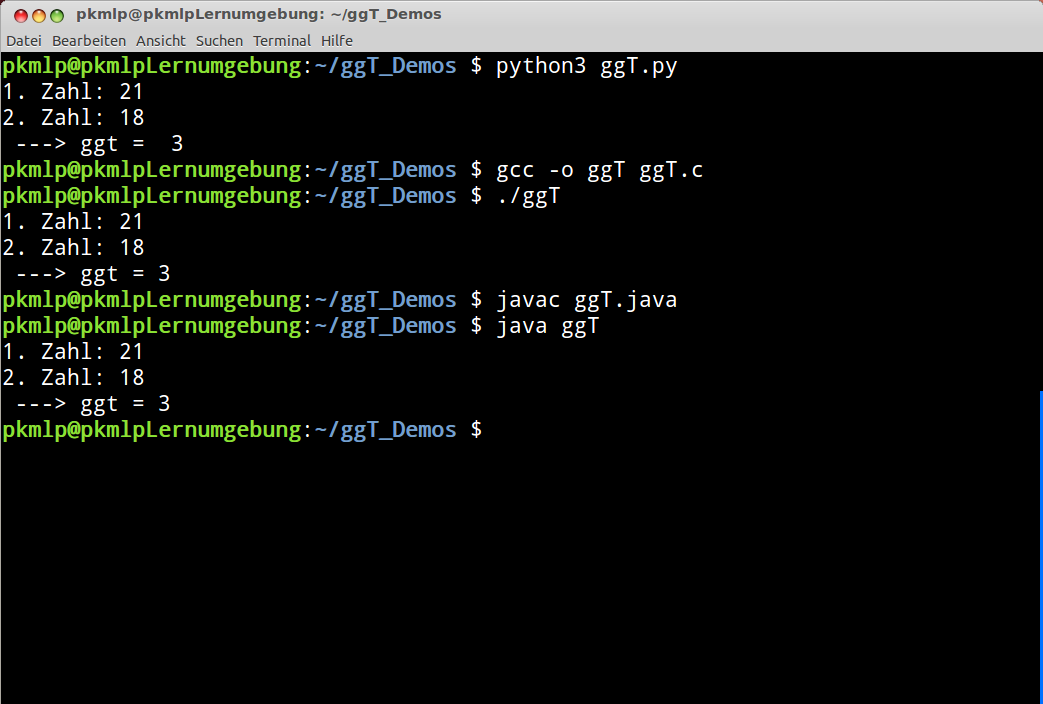
\includegraphics[width=\linewidth]{./screenshots/ggT.png}
  \vspace{-14pt}
  \caption{Beispiel-Output des euklidischen Algorithmus}
  \label{fig:ggT}
\end{figure}

Abbildung \ref{fig:ggT} zeigt die Übersetzung/Kompilierung (sofern notwendig), den Aufruf und den Output der verschiedenen Terminalprogramme.

\textbf{Bitte beachten:} Die Programme sollen lediglich den euklidischen Algorithmus in verschiedenen Programmiersprachen zeigen. Darum wird in den Programmen z.B. keinerlei Überprüfung der Eingabe gemacht. Die verschiedenen Quellcodes sollen vor allem die syntaktischen Unterschiede der Programmiersprachen veranschaulichen. Der Algorithmus ist der Gleiche, die Prinzipien der prozeduralen Programmierung mit 3 Generationssprachen sind die Gleichen, lediglich die Syntax (Schreibweise, Rechtschreibung, etc.) ist unterschiedlich.
